\chapter{Results}
\label{chap:results}
In this chapter we are going to present the obtained results using the previous models, both from a quantitative point of view, by measuring correlation coefficient over predicted data and from a qualitative point of view, by surveying a few listeners with predicted and real performance synthesis. Firstly, in section~\ref{sec:ev_measures} we are going to explain what measures are we going to consider for both results analysis. In section~\ref{sec:features} we are going to apply feature selection in order to see what features are more relevant in order to obtain better prediction for performance actions. Finally in section~\ref{sec:ev_results} we present separately the results from both evaluations, quantitative and qualitative.

\section{Evaluation Measures}
\label{sec:ev_measures}
For the quantitative evaluation we are going to use Correlation Coefficient as evaluation metric. Correlation coefficient tells us how much predicted PAs and computed ones are related. It gives values between -1 and 1, where 0 is no relation, 1 is very strong linear relation and -1 is an inverse linear relation.

\section{Feature Selection}
\label{sec:features}
In figure~\ref{tab:feature_selection} we present the Correlation Coefficients (CC) between predicted and actual Performance Actions for Onset deviation and Energy Ratio. In red we show the accuracy for the whole Train dataset and in blue the results with 10 fold Cross-Validation. The best accuracy (using CV) was obtained with the set containing the first 5 best ranked features.

\begin{table}[ht!]
\centering
 
  \begin{tabular}{  l l p{6cm} }
    \hline
    Dataset & Best Subset & Ranked \\ \hline
    "All (onset\_dev)" & 6, 8, 9, 10, 13, 14, 17 &  6, 17, 8, 13, 10, 14, 9, 5, 27, 26, 24, 31, 20, 18, 16, 35, 23, 25, 32, 29, 12, 11, 22, 4, 19, 15, 33, 3, 7, 34, 21, 2, 30, 28, 1 \\
    "All (energy\_rat) & 6, 7, 9, 20, 21, 24, 27, 32 & 6, 7, 22, 32, 9, 24, 20, 27, 5, 35, 23, 31, 1, 8, 2, 10, 13, 14, 19, 4, 18, 26, 3, 17, 30, 11, 15, 33, 34, 25, 12, 28, 29, 21, 16  \\
    
    \hline
  \end{tabular}

 \caption[Selected Features using Ranker and Best Subset with wrapped Decision Tree]{Selected Features using Best Subset and Ranker with wrapped Decision Tree. Code for descriptors can be found in table~\ref{tab:note_descriptors}.}
  \label{tab:feature_selection}

\end{table}

\begin{figure}[ht!]
\centering
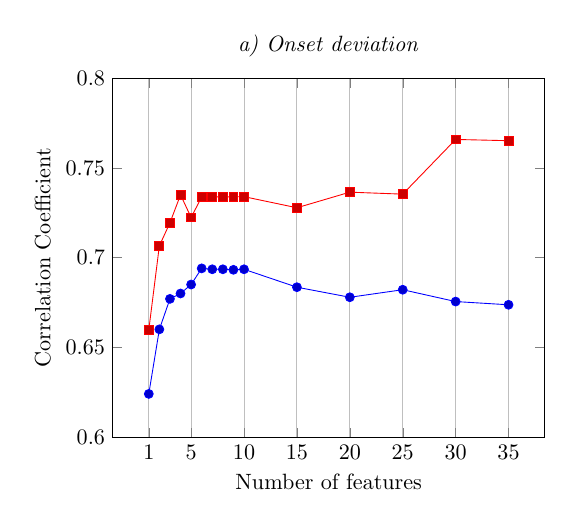
\begin{tikzpicture}[scale=0.8]

\begin{axis}[legend style={font=\scriptsize},
		title={\textit{a) Onset deviation}},
        ylabel={Correlation Coefficient},
        xlabel={Number of features},
        ymin=0.60,ymax=0.80,
        xtick={1,5,10,15,20,25,30,35},
        xmajorgrids]

    \addplot coordinates {(1,0.624) (2,0.660) (3,0.677) (4,0.680) (5,0.685) (6,0.694) (7, 0.6935)  (8, 0.6935) (9,0.6932) (10,0.6935) (15,0.6835) (20, 0.6779)  (25, 0.6821) (30, 0.6755) (35, 0.6737)};
    
    \addplot coordinates {(1, 0.6597) (2, 0.7066)  (3, 0.7194) (4, 0.735) (5, 0.7224) (6, 0.7338) (7, 0.7339) (8, 0.7339) (9, 0.7339) (10, 0.734) (15, 0.7278) (20, 0.7365) (25, 0.7354) (30, 0.7659) (35, 0.7652)};
     
  %  \addlegendentry{Onset\_dev cv10f}
   % \addlegendentry{Energy\_rat cv10f}

\end{axis}
\end{tikzpicture}
\qquad
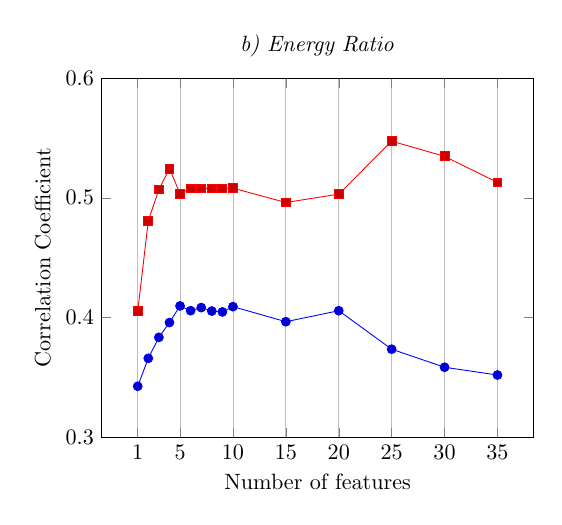
\begin{tikzpicture}[scale=0.8]

\begin{axis}[legend style={font=\scriptsize},
		title={\textit{b) Energy Ratio}},
        ylabel={Correlation Coefficient},
        xlabel={Number of features},
        ymin=0.30,ymax=0.60,
        xtick={1,5,10,15,20,25,30,35},
        xmajorgrids]

     \addplot coordinates { (1,0.3424) (2, 0.3658) (3, 0.3833) (4, 0.3957) (5, 0.4096) (6, 0.4056) (7, 0.4082) (8, 0.4053) (9, 0.4046) (10, 0.4090) (15, 0.3964) (20, 0.4056) (25, 0.3734) (30,0.3583) (35, 0.3518)};
     
     \addplot coordinates { (1, 0.4051) (2, 0.4808) (3, 0.507) (4, 0.5244) (5, 0.5035) (6, 0.5079) (7, 0.5079) (8, 0.5079) (9, 0.5079) (10, 0.5081) (15, 0.4961) (20, 0.5031) (25, 0.5474) (30, 0.5347) (35, 0.5129)};
    
  %  \addlegendentry{CrossValidation 10f}
   % \addlegendentry{Train dataset}

\end{axis}
\end{tikzpicture}

\caption[Results depending on the number of selected features.]{Results depending on the number of selected features according to table~\ref{tab:feature_selection}. Algorithm used: Decision Tree. Shown values correspond to Correlation Coefficients.}
\label{fig:feature_selection}
\end{figure}


\section{Evaluation Results}
\label{sec:ev_results}
In this section we present both quantitative and qualitative results. The proposed approach was quantitatively evaluated by measuring \textit{Correlation Coefficient} (CC) obtained with the models studied and qualitatively evaluated by asking listeners to compare predicted and real performances.

\subsection{Quantitative evaluation}
In table~\ref{tab:results_ml_cv} we show the results comparing different Machine Learning algorithms both with cross-validation and with the whole Train dataset. We present CC for Energy ratio and onset deviation for the whole dataset, for just the best 5 features and also for the best subset of features. As we can see we achieve the best results with Decision Trees and also with just 5 features or the best subset we outperform the normal dataset.

\begin{table}
\centering
\caption[Results comparing different ML models (10 fold Cross-Validation)]{Results comparing different ML models (10 fold Cross-Validation). All datasets correspond to the three datasets merged into one. Shown values correspond to Correlation Coefficients.}
\label{tab:results_ml_cv}
\footnotesize
\begin{tabular} {lcccHcccH}
\\ \hline
\multirow{2}{3cm}{Dataset (feature)} & D.Tree & $k_1NN$ & $k_2NN$ & $k_4NN$ & $k_8NN$ & SVM & ANN & L.Reg \\ 
& cv/train & cv/train & cv/ train & cv/train & cv/train & cv/train & cv/train & cv/train\\\hline

'Darn (energy)' & 0.37/0.53 & 0.18/1 &  0.27/0.78 & 0.27/0.64 &  0.28/0.52 &  0.37/0.55 & 0.26/0.98 & 0.35/0.58 \\
'Darn (onset)' & 0.70/0.87 & 0.35/1 &  0.42/0.83 & 0.48/0.75 & 0.52/0.69 & 0.57/0.68 & 0.47/0.99 & 0.56/0.71  \\
'Suite (energy)' & 0.35/0.59 & 0.24/1 & 0.31/0.77 & 0.33/0.64 & 0.32/0.53 &  0.23/0.38 &  0.17/0.70 & 0.26/0.43 \\
'Suite (onset)' & 0.77/0.88 & 0.28/1 & 0.35/0.80 & 0.37/0.70 & 0.33/0.53 & 0.30/0.40 & 0.29/0.79 & 0.30/0.44 \\
'Suite2 (energy)' & 0.32/0.70 & 0.21/1 & 0.24/0.77 & 0.19/0.59 & 0.17/0.45 & 0.19/0.31 & 0.18/0.66 & 0.19/0.39 \\
'Suite2 (onset)' & 0.83/0.92 & 0.43/1 & 0.48/0.85 & 0.45/0.74 & 0.51/0.85 & 0.44/0.52 & 0.40/0.78 & 0.44/0.55 \\ \hline

'All (energy)' & 0.35/0.51 & 0.22/1 & 0.26/0.78 & 0.27/0.64 & 0.27/0.51 & 0.21/0.33 & 0.23/0.63 & 0.25/0.38 \\
'All (onset)' & 0.67/0.77 & 0.30/1 & 0.36/0.81 & 0.42/0.69 & 0.42/0.60 & 0.39/0.45 & 0.29/0.67 & 0.40/0.47 \\ 
'All (energy)'$_{5 features}$ & 0.41/0.50 & 0.30/1 & 0.37/0.80 & 0.39/0.67 & 0.37/0.57 & 0.14/0.21 & 0.14/0.36 & 0.16/0.23 \\
'All (onset)'$_{5 features}$ & 0.69/0.72 & 0.38/1 & 0.61/0.82 & 0.65/0.79 & 0.65/0.75 & 0.30/0.31 & 0.44/0.43 & 0.31/0.32 \\
'All (energy)'$_{best subset}$ & 0.41/0.51 & 0.30/1 & 0.37/0.79 & 0.38/0.66  & 0.37/0.57  & 0.16/0.21 & 0.15/039 & 0.15/0.23 \\
'All (onset)'$_{best subset}$ & 0.69/0.73 & 0.37/1 & 0.58/0.82 & 0.62/0.78 & 0.64/0.73 & 0.30/0.32 & 0.48/0.48 &  0.31\\

\hline
\end{tabular} 
\footnotesize

\end{table}

%\begin{table}
\centering
\caption[Results comparing different ML models (Train/Test)]{Results comparing different ML models (Train/Test). In this table 66\% of the Dataset has been used as Train and 33\% as Test. Notes has been randomly selected. Shown values correspond to Correlation Coefficients.}
\label{tab:results_ml_tt}
\footnotesize

\begin{tabular} {lcccccccc}
\\ \hline
Dataset (feature) & D.Tree& $k_1NN$ & $k_2NN$ & $k_4NN$ & $k_8NN$ & SVM & ANN & L.Reg \\ \hline
'Darn (energy\_rat)' & 0.44 & 0.14  & 0.21  & 0.23  & 0.31  & 0.32  & 0.34  & 0.35 \\
'Darn (onset\_dev)' & 0.58 & 0.41  & 0.49  & 0.44  & 0.41  & 0.56  & 0.39  & 0.51 \\
'Suite (energy\_rat)' & 0.33 & 0.30  & 0.27  & 0.27  & 0.31  & 0.19  & 0.21  & 0.23 \\
'Suite (onset\_dev)' & 0.67 & 0.32  & 0.43  & 0.44  & 0.42  & 0.35  & 0.39  & 0.39 \\
'Suite2 (energy\_rat)' & 0.31 & 0.21  & 0.17  & 0.15  & 0.06  & 0.11  & 0.23  & 0.12 \\
'Suite2 (onset\_dev)' & 0.79 & 0.37  & 0.51  & 0.48  & 0.56  & 0.45  & 0.44  & 0.49 \\

\hline
\end{tabular}


\footnotesize

\end{table}

In table~\ref{tab:results_mixed} we show the results of training with one dataset and testing with another one. This results are generated using decision tree and artificial neural networks as they show to be the best algorithms in table~\ref{tab:results_ml_cv}. As we can see if we train and test with different performances of the same score we achieve a Correlation Coefficient around 0.3. The poor results in the mixed cases are due to over-fitting the model or to very specific performance actions for each song.
\begin{table}
\centering

\footnotesize
\begin{tabular} {llccHHcc}
\\ \hline

%% & \multicolumn{2}{c}{$k_1NN$}

 \multirow{2}{1cm}{Train} &  \multirow{2}{1cm}{Test} & \multicolumn{2}{c}{D.Tree} & & & \multicolumn{2}{c}{ANN}\\ 
 &  & energy & onset & energy & onset & energy & onset	 \\ \hline
'Darn' & 'Suite' & 0.013 & 0.156 & 0.110 & 0.069 & 0.047 & 0.008 \\
'Darn' & 'Suite2' & 0.091 & 0.183 & 0.018 & 0.177 & 0.033 & 0.075 \\
'Suite' & 'Darn' & 0.017 & 0.140 & 0.333  & 0.11 & 0.107 & 0.032 \\
'Suite' & 'Suite2' &  0.324 & 0.392 & 0.215 & 0.338 & 0.148 & 0.253 \\
'Suite2' & 'Darn' & 0.043 & 0.099 & 0.061 & 0.1672 & 0.079 & 0.027 \\
'Suite2' & 'Suite' & 0.240 &  0.384 & 0.2316 & 0.349 & 0.190 & 0.227 \\
\hline
\end{tabular} 
\footnotesize

\caption[Results mixing songs for Train/Test]{Results mixing songs for Train/Test. Whole song Datasets have been used in order to train or test. Shown values correspond to Correlation Coefficients.}
\label{tab:results_mixed}

\end{table}


\subsection{Qualitative evaluation}

For the qualitative survey, several synthesized pieces obtained by the models were compared to both the score (dead pan synthesis) and the performed (synthesized version) piece. Participants were asked to to guess how "human" they sounded by comparing among them through an on-line survey~\footnote{You can find the survey here: \url{https://marcsiq2.github.io/}}. Results from 15 participants (Figure~\ref{fig:survey}) show that participants perceived the score more "human" than the actual performance and predicted score. However, we obtained similar results among the performed piece and the predicted one, which might indicate that our models predictions are close to actual human performances. Full survey results can be found at Appendix~\ref{app:survey}.

%or the qualitative survey, different MIDIs with the model's predictions are generated and then synthesized. We asked people to guess how "human" they were by comparing them with real performances through an on-line survey~\footnote{You can find the survey here: \url{https://marcsiq2.github.io/}}. We asked them to rate from 0 to 100 how "human" the audios where. Full results can be found at Appendix~\ref{app:survey}. Results from over 10 participants in figure~\ref{fig:survey} show that people find the score more "human" than the actual performance and predicted score. However, as we obtain very similar results for performance and prediction, we can say that our models predict very well the actual human performances. 

Our assumption about why the score synthesis is graded better than the performance or the prediction is that the virtual instrument does not synthesize very well the guitar and when two notes are played with very short inter-onset time it creates very strange artefacts. Moreover, as it is a midi synthesis we are used to hear it very perfect as it always comes from a music score, so introducing those artefacts and time deviations can sound really strange to us, as if the score wasn't well written.

\begin{figure}[ht!]
\caption{Results of the on-line survey with performance, predicted and straight score synthesized midis.}
\label{fig:survey}
\centering
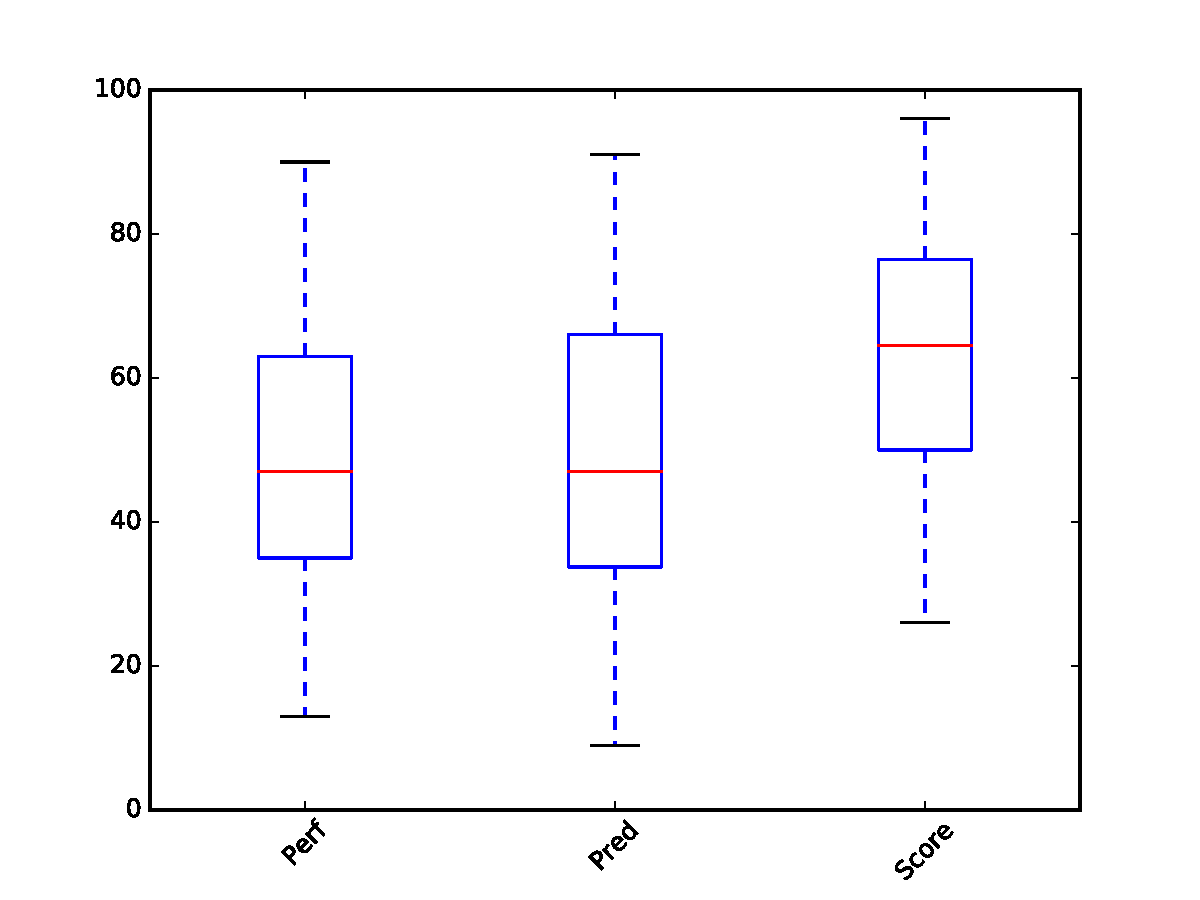
\includegraphics[width=0.7\textwidth]{Figures/survey.pdf}
\end{figure}


\cleardoublepage

